\documentclass[a4paper,12pt]{article}
\usepackage{cmap}
\usepackage[T2A]{fontenc}
\usepackage[utf8]{inputenc}
\usepackage[english,russian]{babel}
\usepackage{listings}
\usepackage{amsmath}
\usepackage{amsfonts}
\usepackage{float}
\usepackage{csquotes}
\usepackage{graphicx}
\usepackage{hyphenat}
\usepackage{xcolor}
\usepackage{hyperref}
\usepackage{mathtools}
\usepackage{upgreek}


\renewcommand{\theequation}{\thesection.\arabic{equation}}


\author{Шерепа Никита}
\title{ThinkDSP. Лабораторная 11. Модуляция и выборка (квантование).}
\date{\today}

\graphicspath{{res/screenshots}}

\begin{document}%
	
	\maketitle
	
	\newpage \tableofcontents
	\newpage \listoffigures
	\newpage \lstlistoflistings
	
	\newpage
	
	\definecolor{dkgreen}{rgb}{0,0.6,0}
	\definecolor{gray}{rgb}{0.5,0.5,0.5}
	\definecolor{mauve}{rgb}{0.58,0,0.82}
	
	\lstset{
		language=Python,                 % выбор ЯП для подсветки 
		basicstyle=\small\sffamily, % размер и начертание шрифта для подсветки кода
		numbers=left,               % где поставить нумерацию строк (слева\справа)
		numberstyle=\tiny,           % размер шрифта для номеров строк
		stepnumber=1,                   % размер шага между двумя номерами строк
		numbersep=5pt,                % как далеко отстоят номера строк от подсвечиваемого кода
		aboveskip=3mm,
		belowskip=3mm,
		showstringspaces=false,
		columns=flexible,
		captionpos=b, 
		basicstyle={\small\ttfamily},
		numbers=left,
		numberstyle=\tiny\color{gray},
		keywordstyle=\color{blue},
		commentstyle=\color{mauve},
		stringstyle=\color{dkgreen},
		breaklines=true,
		breakatwhitespace=true,
		tabsize=3
	}

	\section{Упражение 11.3}
	
	\begin{enumerate}
		
		\item{Задание}
		
		К примеру "Соло на барабане" примените фильтр НЧ до выборки, а затем, опять же с помощью фильтра НЧ, удалите спектральные копии, вызванные выборкой. Результат должен быть идентичен отфильтрованному сигналу.
		
		\item{Ход работы}
		
		Возьмем ритмичное джангл-соло на барабанах.
		\begin{lstlisting}[caption=Джангл-соло]
			wave = read_wave('res/263868__kevcio__amen-break-a-160-bpm.wav')
			wave.normalize()
			wave.plot()
		\end{lstlisting}
		\begin{figure}[H]
			\centering
			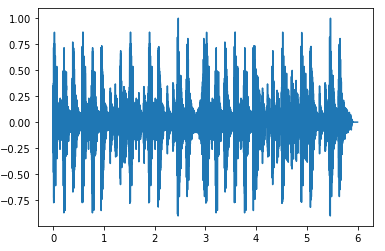
\includegraphics[width=0.75\textwidth]{3_1.png}
			\caption{Джангл-соло}
			\label{fig:3.1}
		\end{figure}
		
		Построим спектр
		\begin{lstlisting}[caption=Спектр]
			spectrum = wave.make_spectrum(full=True)
			spectrum.plot()
		\end{lstlisting}
		\begin{figure}[H]
			\centering
			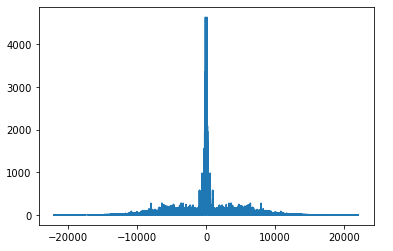
\includegraphics[width=0.75\textwidth]{3_2.png}
			\caption{Спектр}
			\label{fig:3.2}
		\end{figure}
		
		Уменьшим частоту дискретизации в 3 раза
		\begin{lstlisting}[caption=Уменьшаем частоту дискретизации]
			factor = 3
			framerate = wave.framerate / factor
			cutoff = framerate / 2 - 1
		\end{lstlisting}
		
		Теперь немного сгладим спектр: удалим частоты выше новой частоты свертки, которая равна частоте кадров / 2
		\begin{lstlisting}[caption=Сглаживаем]
			spectrum.low_pass(cutoff)
			spectrum.plot()
		\end{lstlisting}
		\begin{figure}[H]
			\centering
			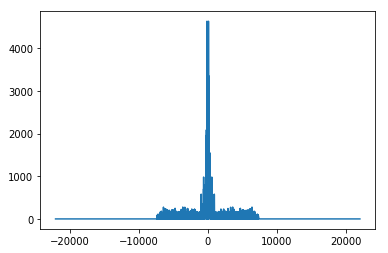
\includegraphics[width=0.75\textwidth]{3_3.png}
			\caption{Удалили частоты}
			\label{fig:3.3}
		\end{figure}
	
		После фильтрации запись звучит веьсма атмосферно - немного приглушенно, как олдскульный джангл-микс из платстинки в каком-нибудь музыкальном магазине 90х годов.
		
		Вот функция, имитирующая процесс дискретизации
		\begin{lstlisting}[caption=Функция \texttt{sample()}]
			from thinkdsp import Wave
			
			def sample(wave, factor):
				ys = np.zeros(len(wave))
				ys[::factor] = np.real(wave.ys[::factor])
				return Wave(ys, framerate=wave.framerate) 
		\end{lstlisting}
		
		Применим к нашей записи
		\begin{lstlisting}[caption=Применяем \texttt{sample()}]
			sampled = sample(filtered, factor)
			sampled.make_audio()
		\end{lstlisting}
		
		Результат содержит очень заметные копии спектра около 20 кГц. Отобразим их.
		\begin{lstlisting}[caption=Отображаем результат]
			from thinkdsp import Wave
			
			def sample(wave, factor):
			ys = np.zeros(len(wave))
			ys[::factor] = np.real(wave.ys[::factor])
			return Wave(ys, framerate=wave.framerate) 
		\end{lstlisting}
		\begin{figure}[H]
			\centering
			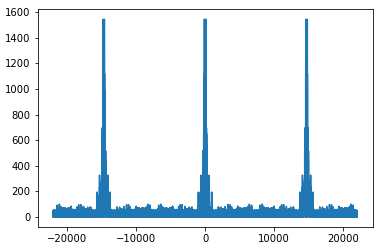
\includegraphics[width=0.75\textwidth]{3_4.png}
			\caption{Результат}
			\label{fig:3.4}
		\end{figure}
		
		 
		Избавимся от спектральных копий, снова применив фильтр сглаживания
		\begin{lstlisting}[caption=Избавляемся от спектральных копий]
			sampled_spectrum.low_pass(cutoff)
			sampled_spectrum.plot()
		\end{lstlisting}
		\begin{figure}[H]
			\centering
			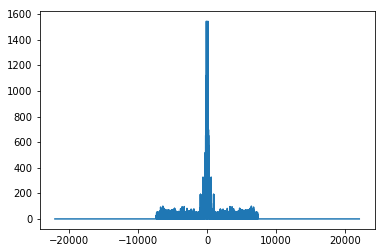
\includegraphics[width=0.75\textwidth]{3_5.png}
			\caption{Без копий}
			\label{fig:3.5}
		\end{figure}
	
		Мы только что потеряли половину энергии в спектре, но мы можем масштабировать результат, чтобы вернуть его
		\begin{lstlisting}[caption=Масштабируем результат]
			sampled_spectrum.scale(factor)
			spectrum.plot()
			sampled_spectrum.plot()
		\end{lstlisting}
		\begin{figure}[H]
			\centering
			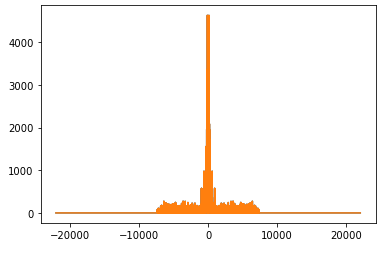
\includegraphics[width=0.75\textwidth]{3_6.png}
			\caption{Масштабируем результат}
			\label{fig:3.6}
		\end{figure}
	
		Вычислим разницу между спектром до и после выборки
		\begin{lstlisting}[caption=Вычисляем разницу]
			spectrum.max_diff(sampled_spectrum)
			
			Output
			1.8189894035458565e-12
		\end{lstlisting}
		
		Разница мала и равна 1.8189894035458565e-12
		
		После фильтрации и масштабирования преобразуем обратно в волну
		\begin{lstlisting}[caption=Обратно в волну]
			interpolated = sampled_spectrum.make_wave()
			interpolated.make_audio()
		\end{lstlisting}
		
		Теперь сравним интерполированную волну и отфильтрованную волну
		\begin{lstlisting}[caption=Отфильтрованная волна]
			filtered.plot()
		\end{lstlisting}
		\begin{figure}[H]
			\centering
			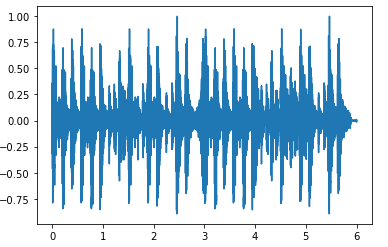
\includegraphics[width=0.75\textwidth]{3_7.png}
			\caption{Отфильтрованная волна}
			\label{fig:3.7}
		\end{figure}
		\begin{lstlisting}[caption=Интерполированная волна]
			interpolated.plot()
		\end{lstlisting}
		\begin{figure}[H]
			\centering
			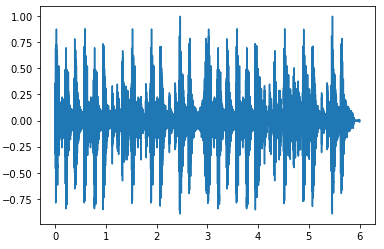
\includegraphics[width=0.75\textwidth]{3_8.png}
			\caption{Интерполированная волна}
			\label{fig:3.8}
		\end{figure}
	
		Вычислим разницу
		\begin{lstlisting}[caption=Разница]
			filtered.max_diff(interpolated)
			
			Output
			5.56290642113787e-16
		\end{lstlisting}
		
		Видим, что графики похожи, а разница крайне мала и равна 5.56290642113787e-16
		
		
		\section{Вывод}
		
		В результате выполнения работы получены навыки работы с выборкой. Выяснено, что если применить к сигналу фильтр НЧ до выборки, и сравнить его с таким же сигналом, но в которому применили выборку и затем удалили спектральные копии, то результаты будут идентичны.
		
	\end{enumerate}

\end{document}